\documentclass[t]{beamer}
\usefonttheme{serif}

\usepackage{amsmath,amsthm,amssymb,amsfonts,amscd,mathrsfs,amsxtra,multirow,kotex,mathtools,gensymb,textcomp,lipsum,tikz,verbatim,color,soul,courier,mdframed,xcolor}
\usepackage[normalem]{ulem}
\usetikzlibrary{calc,matrix,arrows,chains,positioning,scopes}
\usepackage{pdfpages,cancel}

\theoremstyle{plain}
\newtheorem{thm}{Theorem}[section]
\newtheorem{prop}[thm]{Proposition}

\theoremstyle{definition}
\newtheorem{defn}[thm]{Definition}
\newtheorem{exmp}[thm]{Example}
\newtheorem{excs}[thm]{Exercise}
\newtheorem{rem}[thm]{Remark}
\newtheorem{prob}[thm]{Problem}
\newtheorem{cor}[thm]{Corollary}

\newcommand \tr[1]{\textcolor{red}{#1}}
\newcommand{\tikzmark}[1]{\tikz[overlay,remember picture] \node (#1) {};}
\newcommand{\varep}{\varepsilon}
\newcommand{\DrawBox}[1][]{%
    \tikz[overlay,remember picture]{
    \draw[red,#1]
      ($(left)+(-0.2em,0.9em)$) rectangle
      ($(right)+(0.2em,-0.3em)$);}
}

\newcommand{\tikzmarkk}[2]{
    \tikz[overlay,remember picture,baseline] 
    \node[anchor=base] (#1) {$#2$};
}
\newcommand*\circled[1]{\tikz[baseline=(char.base)]{
            \node[shape=circle,draw,inner sep=2pt] (char) {#1};}}

\tikzset{join/.code=\tikzset{after node path={%
\ifx\tikzchainprevious\pgfutil@empty\else(\tikzchainprevious)%
edge[every join]#1(\tikzchaincurrent)\fi}}}

\tikzset{>=stealth',every on chain/.append style={join},
         every join/.style={->}}
\tikzstyle{labeled}=[execute at begin node=$\scriptstyle,
   execute at end node=$]

\newenvironment<>{proofs}[1][\proofname]{%
   \par
   \def\insertproofname{#1\@{.}}%
   \usebeamertemplate{proof begin}#2}
 {\usebeamertemplate{proof end}}
 

\addtobeamertemplate{navigation symbols}{}{%
    \usebeamerfont{footline}%
    \usebeamercolor[fg]{footline}%
    \hspace{1em}%
    \raisebox{2pt}[0pt][0pt]{\insertframenumber/\inserttotalframenumber}
}
\setbeamercolor{footline}{fg=blue}
\setbeamerfont{footline}{series=\bfseries}
\title[]{SE102:Multivariable Calculus}

\author[]{Hyosang Kang\inst{1}}

\institute[]{\inst{1}Division of Mathematics\\ School of Interdisciplinary Studies\\ DGIST}

\date[]{Lecture 06\\
Line and Surface Integrals}

\begin{document}

\begin{frame}
\titlepage
\end{frame}

\begin{frame}
\begin{defn}
Given an interval $I\subset\mathbf R$, a curve $C$ parametrized by $c:I\rightarrow\mathbf R^n$
	\[c(t)=(x^0(t),x^1(t),\cdots,x^{n-1}(t))\]
is \textbf{piecewise differentiable} if all coordinate functions $x^i(t)$ are 
of $\mathcal C^n$ class on the interval $I$ except for finitely many points.
\end{defn}
\begin{defn}
Let $C$ be a piecewise differentiable curve on $\mathbf R^2$ parametrized by 
$c:[a,b]\to\mathbf R^2$ and $c'(t)=(x'(t),y'(t))$ be the velocity vector.
Given a function $f(x,y)$ defined on the curve $C$,
the \textbf{line integral} of $f(x,y)$ along $C$ is defined as
	\[\int_Cfds=\int_a^bf(c(t))\Vert c'(t)\Vert dt.\]
\end{defn}
\end{frame}

\begin{frame}
\begin{prop}
The line integral $\displaystyle \int_C f ds$ does not depend on the parametrization of $C$.
\end{prop}
\begin{proof}
Let $c:[a,b]\to\mathbf R^2$ be a parametrization of $C$.
Let $h:[c,d]\to[a,b]$ be a one-to-one correspondence which gives a \emph{re-parametrization} $c\circ h$ of $C$.
Let us write $t = h(\tau)$. Then
    \begin{align*}
        \int_c^df(c\circ h(\tau)) \cdot \Vert(c\circ h)'(\tau)\Vert d\tau 
        &= \int_c^d f(c(t)) \cdot \Vert c'(t)\Vert \cdot \Vert h'(\tau)\Vert d\tau \\
        &= \int_a^b f(c(t)) \cdot \Vert c'(t)\Vert dt
    \end{align*}
\end{proof}
\end{frame}

\begin{frame}
\begin{exmp}
Compute the line integral \[\displaystyle\int_C (2+x^2y)ds\]
where $C$ is the unit circle centered at the origin with counter clockwise orientation.
\end{exmp}
\end{frame}

\begin{frame}
\begin{defn}
Let $S$ be a suface in $\mathbf R^3$ and $D$ be the region in $\mathbf R^2$.
A map $X:D\rightarrow S$
	\[X(u,v)=(x(u,v),y(u,v),z(u,v))\]
is called the \textbf{parametrization} of the surface $S$ if
it is a one-to-one correspondence and
every partial derivative of $x,y,z$ is continuous on $D$.
\end{defn}
\begin{exmp}
Find a parametrization of $S=\{(x,y,z)\,|\,x^2+y^2-z^2=1\}$.
\end{exmp}
\end{frame}

\begin{frame}
\begin{defn}
Let $f(x,y,z)$ be a function defined on a surface $S$.
which is parametrized by $X:D\rightarrow S$.
The \textbf{surface integral} of $f$ on $S$ is defined by
	\[\iint_SfdS=\iint_D(f\circ X)(u,v)\Vert X_u\times X_v\Vert dudv.\]
\end{defn}

\begin{exmp}
Let $S$ be the surface defined by the graph of $z=\sqrt{x^2+y^2}$ 
over the disk $x^2+y^2\le 1$. Compute $\displaystyle\iint_S zdS$.
\end{exmp}
\end{frame}
\begin{frame}
\begin{defn}\label{defn-Jacobian}
Let $D,R$ be regions in $\mathbf R^n$.
A map $\mathbf T:R\to D$ is called a \textbf{transformation} 
if it is differentiable and one-to-one.
The determinant of the differential of $\mathbf T$ 
is called the \textbf{Jacobian} of $T$ and is denoted by 
	\[J_{\mathbf T} = \det \mathbf{dT}.\]
When the variables are explicitly presented as
$T(u^0,\cdots,u^{n-1}) = (x^{0},\cdots,x^{n-1})$, 
the Jacobian is also denoted as
	\[J_{\mathbf T} = \det\frac{\partial(x^0,\cdots,x^{n-1})}{\partial(u^0,\cdots,u^{n-1})}.\]
\end{defn}
\end{frame}

\begin{frame}
\begin{thm}[Integration by substitution]
Let $T:R\to D$ be a transformation, 
and $f(x,y)$ be a continuous function defined on $D$.
Then
	\[\iint_Df(x,y)dxdy=\iint_R(f\circ T)(u,v)|J_T|dudv.\]
\end{thm}
\begin{rem}
It is useful to remember the subsitution rule as:
	$$\iint_Df(x,y)dxdy
	= \iint_R(f\circ T)(u,v)\left|\frac{\partial(x,y)}{\cancel{\partial(u,v)}}\right|\cancel{dudv}$$
Also, the Jacobian of the inverse $\mathbf T^{-1}(x,y)=(u(x,y),v(x,y))$ is
	$$J_{\mathbf T^{-1}}=\left|\frac{\partial(u,v)}{\partial(x,y)}\right|
	=\frac{1}{J_{\mathbf T}}=\frac{1}{\left|\frac{\partial(x,y)}{\partial(u,v)}\right|}$$
\end{rem}
\end{frame}

\begin{frame}
\begin{exmp}
Compute
	\[\iint_D |x|e^{-x^2-y^2}dxdy\]
where $D=\{(x,y)\,|\,x^2+y^2\le1\}$.
\end{exmp}
\end{frame}

\begin{frame}
\begin{rem}
The integration by substitution works on triple integral as well.
Let $V,W$ be regions in $\mathbf R^3$.
A differentiable one-to-one function $T:W\to V$ 
	\[T(u,v,w) = (x(u,v,w),y(u,v,w),z(u,v,w))\]
is called a \textbf{transformation}.
Let $f(x,y,z)$ be a continuous function on $V$.
Then
	\[\iiint_Vf(x,y,z)dxdydz=\iiint_W(f\circ T)(u,v,w)|J_T|dudvdw.\]
\end{rem}
\end{frame}

\begin{frame}
\begin{exmp}
Compute the volume between two cylinders $x^2+y^2\le 1$, $y^2+z^2\le 1$.
	\begin{figure}
	\begin{center}
	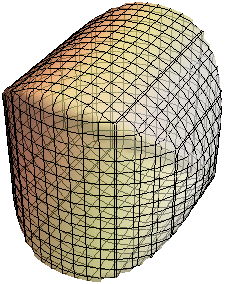
\includegraphics[scale=.25]{image/lnsec10-1}
	\end{center}
    \end{figure}
\end{exmp}
\end{frame}

\begin{frame}
\begin{exmp}
Compute
	\[\iiint_V\sqrt{x^2+y^2+z^2}e^{x^2+y^2+z^2}dxdydz\]
where $V$ is the region between the spheres $x^2+y^2+z^2=a^2$ and $x^2+y^2+z^2=b^2$ ($0<a<b$).
\end{exmp}
\end{frame}

\begin{frame}
\begin{defn}
Let $V$ be a $n$-dimensional vector space.
A \textbf{vector field} $\mathbf F:\mathbf R^n\to V$
is a map  which assign a vector in a vector space $V$
to each point in the space $\mathbf R^n$.
For the simplicity, we call $\mathbf F$ as $n$-dimensional vector field.
\end{defn}

\begin{defn}
Let $\mathbf F:\mathbf R^n\to V$ be a $3$-dimensional vector field defined by
	\[\mathbf F(x,y,z) = (P(x,y,z), Q(x,y,z), R(x,y,z)).\]
The \textbf{curl} $\nabla\times \mathbf F$ and 
the \textbf{divergence} $\nabla\cdot\mathbf F$ is defined by
\begin{align*}
	\nabla\times\mathbf F &= (R_y-Q_z,P_z-R_x,Qx-P_y), \\
	\nabla\cdot\mathbf F &= P_x+Q_y+R_z.
\end{align*}
\end{defn}
\end{frame}

\begin{frame}
\begin{rem}
The curl of a vector field is a vector field, while the divergence is 
a scalar function. It is convenient to remember the formula 
of the curl $\nabla\times \mathbf F$ as
	\[\nabla\times\mathbf F = \left|\begin{matrix} i & j & k \\ \partial/\partial_x & \partial/\partial_y & \partial/\partial_z \\ P & Q & R \end{matrix}\right|.\] 
Also, some defines the curl and divergence of $2$-dimensional vector fields as well.
For $2$-dimensional vector field $\mathbf F(x,y)=(P(x,y), Q(x,y))$,
the curl is a \emph{scalar}
	\[\textup{curl}\mathbf F = Q_x - P_y,\]
and the divergence is  
	\[\textup{div}\mathbf F = P_x + Q_y.\]
\end{rem}
\end{frame}

\begin{frame}
\begin{thm}
Let $f,g$ be $3$-dimensional functions
and $\mathbf F$, $\mathbf G$ be $3$-dimensional vector fields. 
The following properties hold.
\begin{enumerate}
\item $\nabla\times(\nabla f)=0$ 
\item $\nabla\cdot(\nabla\times\mathbf F)=0$
\item $\nabla\cdot(\mathbf F+\mathbf G)=\nabla\cdot\mathbf F+\nabla\cdot\mathbf G$
\item $\nabla\times(\mathbf F+\mathbf G)=\nabla\times\mathbf F+\nabla\times\mathbf G$
\item $\nabla\cdot(f\mathbf F)=f\nabla\cdot\mathbf F+\mathbf F\cdot\nabla f$
\item $\nabla\times(f\mathbf F)=f\nabla\times\mathbf F+\nabla f\times\mathbf F$
\item $\nabla\cdot(\mathbf F+\mathbf G)=\mathbf G\cdot(\nabla\times\mathbf F)-\mathbf F\cdot(\nabla\times\mathbf G)$
\item $\nabla\cdot(\nabla f\times\nabla g)=0$
\item Denote $\nabla^2=\nabla\cdot\nabla$. Then
	\[\nabla\times(\nabla\times\mathbf F)=\nabla(\nabla\cdot\mathbf F)-\nabla^2\cdot\mathbf F\]
\end{enumerate}
\end{thm}
\end{frame}

\begin{frame}
\begin{defn}
Let $C$ be a curve in $\mathbf R^n$ parametrized by 
$\mathbf c:[a,b]\to\mathbf R^n$.
The \textbf{line integral} of $\mathbf F$ on $C$, 
denoted by $\displaystyle\int_C\mathbf F\cdot d\mathbf s$, is defined by
	\[\int_C\mathbf F\cdot d\mathbf s 
	= \int_a^b\mathbf F\circ \mathbf c(t)))\cdot \mathbf c'(t)dt.\]
When $\mathbf c(a)=\mathbf c(b)$, the curve is said to be \textbf{closed}.
The line integral on a closed curve is denoted by
	\[\oint_C\mathbf F\cdot d\mathbf s.\]
\end{defn}	
\end{frame}

\begin{frame}
For $2$-dimensional vector field $\mathbf F = (P,Q)$,
the line integral is denoted by
	\[\int_C\mathbf F\cdot d\mathbf s = \int_C Pdx + Qdy.\]
For $3$-dimensional vector field $\mathbf F = (P,Q,R)$,
the line integral is denoted by
	\[\int_C\mathbf F \cdot d\mathbf s = \int_C Pdx + Qdy + Rdz.\]
\begin{exmp}
Let $\mathbf A = \displaystyle 
	\left(-\frac{y}{x^2+y^2},\frac{x}{x^2+y^2}\right)$.
Compute the line integral $\displaystyle \oint_C\mathbf A\cdot d\mathbf s$
where $C$ is a unit circle parametrized by counter-clockwise direction.
\end{exmp}
\end{frame}

\begin{frame}
\begin{defn}
Let $X:D\rightarrow S$ be a parametrization of $S$.
When the vector field $\mathbf n$ defined by
	$$\mathbf n
	=\frac{\mathbf X_u\times \mathbf X_v}{\Vert \mathbf X_u\times \mathbf X_v\Vert }$$
is continuous, $\mathbf n$ is called an \textbf{orientation} of $S$.
If a surface admits a parametrization with an orientation,
then we say $S$ is \textbf{orientable}.
\end{defn}
\begin{defn}
Let $\mathbf F$ be a $3$-dimensional vector field
defined on an orientable surface $S$ parametrized by $X:D\to S$.
Then \textbf{surface integral} of $\mathbf F$ over $S$ with respect to
an orientation $\mathbf n$,
denoted by $\displaystyle\iint_S\mathbf F\cdot d\mathbf S$, is defined by
	\[\iint_S\mathbf F\cdot d\mathbf S 
	= \iint_D(\mathbf F\circ X) \cdot\mathbf ndA.\]
\end{defn}
\end{frame}

\begin{frame}
\begin{exmp}
Pick an orientation of a unit sphere and 
compute the surface integral of $\mathbf F = \displaystyle
\frac{(x,y,z)}{x^2+y^2+z^2}$.
\end{exmp}	
\end{frame}

\begin{frame}
\begin{prob}
Let $f(x,y)$ be a function defined on a curve $C$.
Explain the meaning of the line integral $\displaystyle \int_Cfds$ 
in the following senses:
\begin{enumerate}
	\item when $f(x,y)$ is a density at $(x,y)$ on the curve $C$,
	the integral $\displaystyle\int_C fds$ is the mass of $C$;
	\item the integral $\displaystyle\int_C fds$ is the area of 
	the section of the graph $z=f(x,y)$ over the curve $C$.
\end{enumerate}
\end{prob}
\end{frame}

\begin{frame}
\begin{prob}
Let $\mathbf F$, $\mathbf G$ be $3$-dimensional vector fields.
Show that the following properties hold. 
\begin{enumerate}
	\item $\nabla\cdot(\mathbf F\times\mathbf G)=\mathbf G\cdot(\nabla\times\mathbf F)-\mathbf F\cdot(\nabla\times\mathbf G)$
	\item $\nabla\times(\nabla\times\mathbf F)=\nabla(\nabla\cdot\mathbf F)-\nabla\cdot \nabla\cdot\mathbf F$
	\item $\nabla\times(\mathbf F\times\mathbf G) = (\nabla\cdot\mathbf G)\mathbf F - (\nabla\cdot \mathbf F)\mathbf G + (\mathbf G\cdot\nabla)\cdot \mathbf F - (\mathbf F\cdot\nabla)\cdot \mathbf G$
\end{enumerate}
\end{prob}
\end{frame}

\begin{frame}
\begin{prob}
Find the area of the region bounded by three cylinders
$x^2+y^2\le 1$, $y^2+z^2\le 1$, and $x^2+z^2\le 1$.
\begin{center}
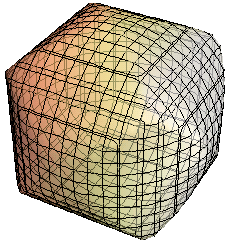
\includegraphics[scale=.25]{image/lnsec10-2}
\end{center}
\end{prob}
\end{frame}

\end{document}